%%%%%%%%%%%%%%%%%%%%%%%%%%%%%%%%%%%%%%%%%%%%%%%%%%%%%%%%%%%%%%%
%
% Welcome to Overleaf --- just edit your LaTeX on the left,
% and we'll compile it for you on the right. If you open the
% 'Share' menu, you can invite other users to edit at the same
% time. See www.overleaf.com/learn for more info. Enjoy!
%
%%%%%%%%%%%%%%%%%%%%%%%%%%%%%%%%%%%%%%%%%%%%%%%%%%%%%%%%%%%%%%%
\documentclass[12pt]{article}

\usepackage{lipsum} %dont know
\usepackage{geometry}
\geometry{top=2.5cm, left=2.6cm, right=2.1cm}
\usepackage{graphicx}
\usepackage{float}
\graphicspath{{images/}}
\usepackage{mathtools}
\usepackage{listings}
\lstset{language=Verilog, breaklines=true}
\usepackage{underscore}
\usepackage[utf8]{inputenc}



\begin{document}

\begin{titlepage}
  \begin{center}
  
\vspace*{0.5cm} 
  \Large{ISTANBUL TECHNICAL UNIVERSITY
COMPUTER ENGINEERING DEPARTMENT}

\vspace{2cm}
  \huge{\textbf{BLG222E}}\\
  \huge{\textbf{COMPUTER ORGANIZATION PROJECT 1 REPORT}}

\vspace{3cm}
  \Large{\textbf{Group Members:}}\\
  150200011 Çağla Mıdıklı\\
  150210049 Feyza Sarı\\
  820210305 Berna Karatay 
  
\vfill
  \Large{\textbf{12 APRIL 2023}}  
  
  \end{center}

  \end{titlepage}

%contents 
\tableofcontents
\thispagestyle{empty}  
\clearpage
\setcounter{page}{1}

\section{Introduction}
In this project we designed n-bit register, 16-bit IR register, register file(RF), address register file(ARF), arithmetic logic unit(ALU) and we implement a ALU system.


\section{Project}


\subsection{Part-1}
An n-bit register is designed in this section. Two 2-bit control signals (FunSel) and an enable input govern four of this register's possibilities.While the value of enable input is 0,  the register returns the same value regardless of the funsel's value. The value of the funsel variable is subject to various actions if the enable input value is 1. These operations are, in order, clear, load, decrement, and increment.We defined n as parameters while writing this module in order to easily access the registers with different bit values that we need in other modules. We set our output's equivalence to 0 when funsel is 0. The output and input are equivalent when funsel is 1. Its previous value is reduced by one when it is multiplied by two. When it reaches 3, it adds one to its previous number. We repeat running the always block each time the clock signal is activated.

\begin{figure}[H]
    \centering
    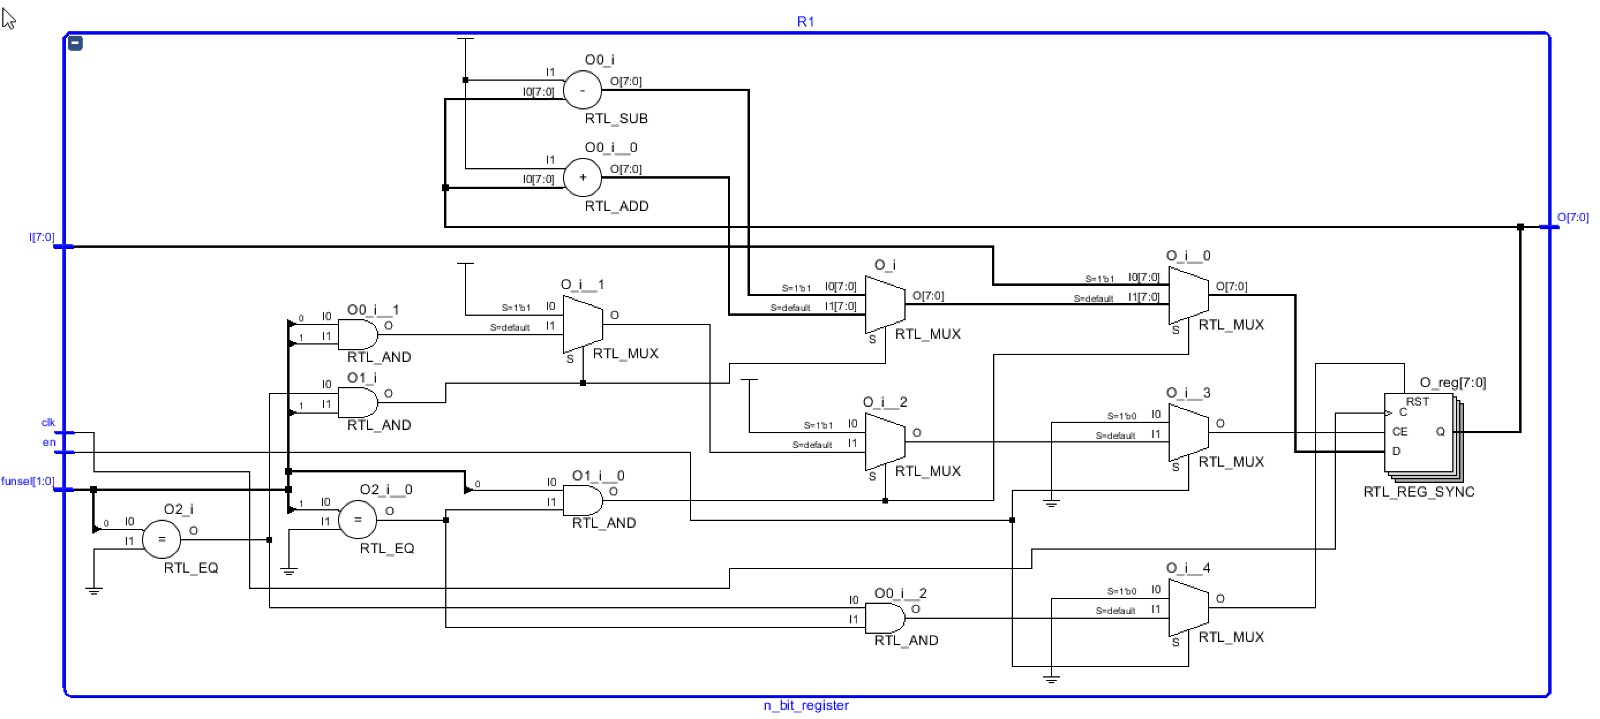
\includegraphics[width=5in]{8bit1.jpg}
    \caption{an example for 8-bit register}
    \label{fig:part1} %referans 
\end{figure}

The module n\_bit\_register has the following inputs:
\begin{itemize}
    \item en: an input signal that enables the register operation when high.
    \item funsel: a 2-bit input signal that selects the function to be performed by the register.
    \item I: an n-bit input signal that is used as input to the register.
    \item clk: the clock input signal.
\end{itemize}

O is a n-bit output signal that represents the output of the register.

\clearpage


Implementation of this module in Verilog shown in below:

\vspace{0.5cm}
\begin{lstlisting}
module n_bit_register #(parameter n = 8)(
    
    input en, 
    input [1:0]FunSel,
    input [n-1:0]I,
    output reg [n-1:0]O,
    input clk
    );
    
    
    always @(posedge clk)begin
            
            if (en == 0) begin
                
            end else if(FunSel== 00)
            begin
                O = 0;
                
            end else if(FunSel == 01)
            begin
                O = I;
               
            end else if(FunSel == 10)
            begin
                O = O - 1;
                
            end else if(FunSel == 11)
            begin
                O = O + 1;
            end
            
            
        end
        endmodule
\end{lstlisting}

\clearpage
        
\subsection{Part-2}
In this part, we designed register files.

\subsubsection{Part-2a)}
In answer to question two, part a, we defined a register that produces a 16-bit output. Three inputs are used to control this register. These inputs are funsel, enable and low\_high. The value doesn't change when enable is set to 0. Funsel and low\_high variables are verified when enable is 1. When enable is 1 and funsel is 0, our value will be 0.

Our input is loaded into bits 0–7 if our l\_h value is 0 and funsel is set to 1 and this part referred to as the lower half. Our input is loaded into bits 8–15 if funsel is 01 and l\_h is 1 and this part referred to as the high half. Funsel is equal 10 to reduce the value by 1. The value is decreased by one when funsel is 11. We repeat running the always block each time the clock signal is activated.

\vspace{0.5cm}
\begin{figure}[H]
    \centering
    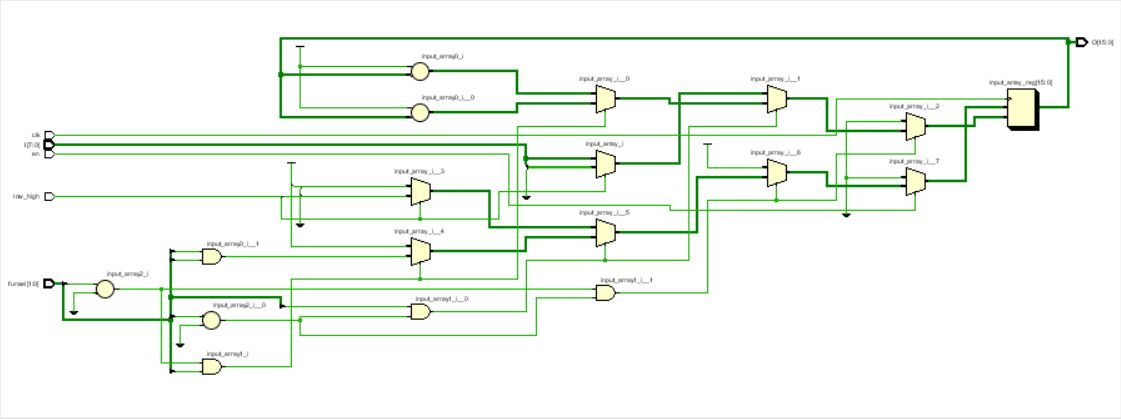
\includegraphics[width=6in]{2a.jpg}
    \caption{Figure for part-2a}
    \label{fig:part2a}
\end{figure}

The module two\_a has the following inputs:
\begin{itemize}
    \item en: A single-bit input used to enable or disable the register.
    \item clk: A single-bit input used as the clock signal for the register.
    \item funsel: A two-bit input that determines the operation to be performed on the register.
    \item I: An 8-bit input data to be stored in the register.
    \item low\_high: A single-bit input used to select between storing the input data in the lower 8 bits or the higher 8 bits of the register.
\end{itemize}

\clearpage

Implementation of this module in Verilog shown in below:
 
\vspace{0.5cm}
\begin{lstlisting}
module two_a(
            input en,clk,
            input [1:0]funsel,
            input [7:0]I,
            input low_high,
            output reg [15:0]O
            );
         
            always @(posedge clk)begin
                    
                    if (en == 0) begin
                    O = O;
                    end else if(funsel[0] == 0 && funsel[1] == 0)
                    begin
                        O = 0;
                        
                    end else if(funsel[0] == 1 && funsel[1] == 0)
                    begin
                        if(low_high == 0)
                        begin
                            O[7:0] = I;
                        end else if(low_high == 1)
                        begin
                              O[15:8] = I;
                        end
                        
                    end
                    else if(funsel[0] == 0 && funsel[1] == 1)
                    begin
                        O = O - 1;
                        
                    end else if(funsel[0] == 1 && funsel[1] == 1)
                    begin
                        O = O + 1;
                    end
                    
                end
                
                endmodule  
\end{lstlisting}              

\clearpage


\subsubsection{Part-2b)}
This module implementing a Register File (RF) using eight n-bit registers and two 8-to-1 multiplexers. 7 inputs are used to control this register file:
\begin{itemize}
    \item IN is 8-bit data input. All of the n-bit registers are connected to the input IN.
    \item O1Sel and O2Sel are output selection inputs. The 8-to-1 multiplexers output is selected by the 3-bit O1Sel and O2Sel signals.
    \item RSel and TSel are to determine which registers are enable
    \item  The 2-bit FunSel signal determines the function to be applied to the data, which is determined by the RSel and TSel signals.   
    \item The last one is clock signal for registers.
    \end{itemize}

The 4-bit signals RSel and TSel are used to choose the data source for the function defined by FunSel. The multiplexers' 8-bit outputs, designated by O1Sel and O2Sel respectively, are RF\_AOut and RF\_BOut. 
Overall, this module allows for multiple sources of data to be selected and operated on by the specified function before being output to the destination registers selected by O1Sel and O2Sel.

\begin{figure}[H]
    \centering
    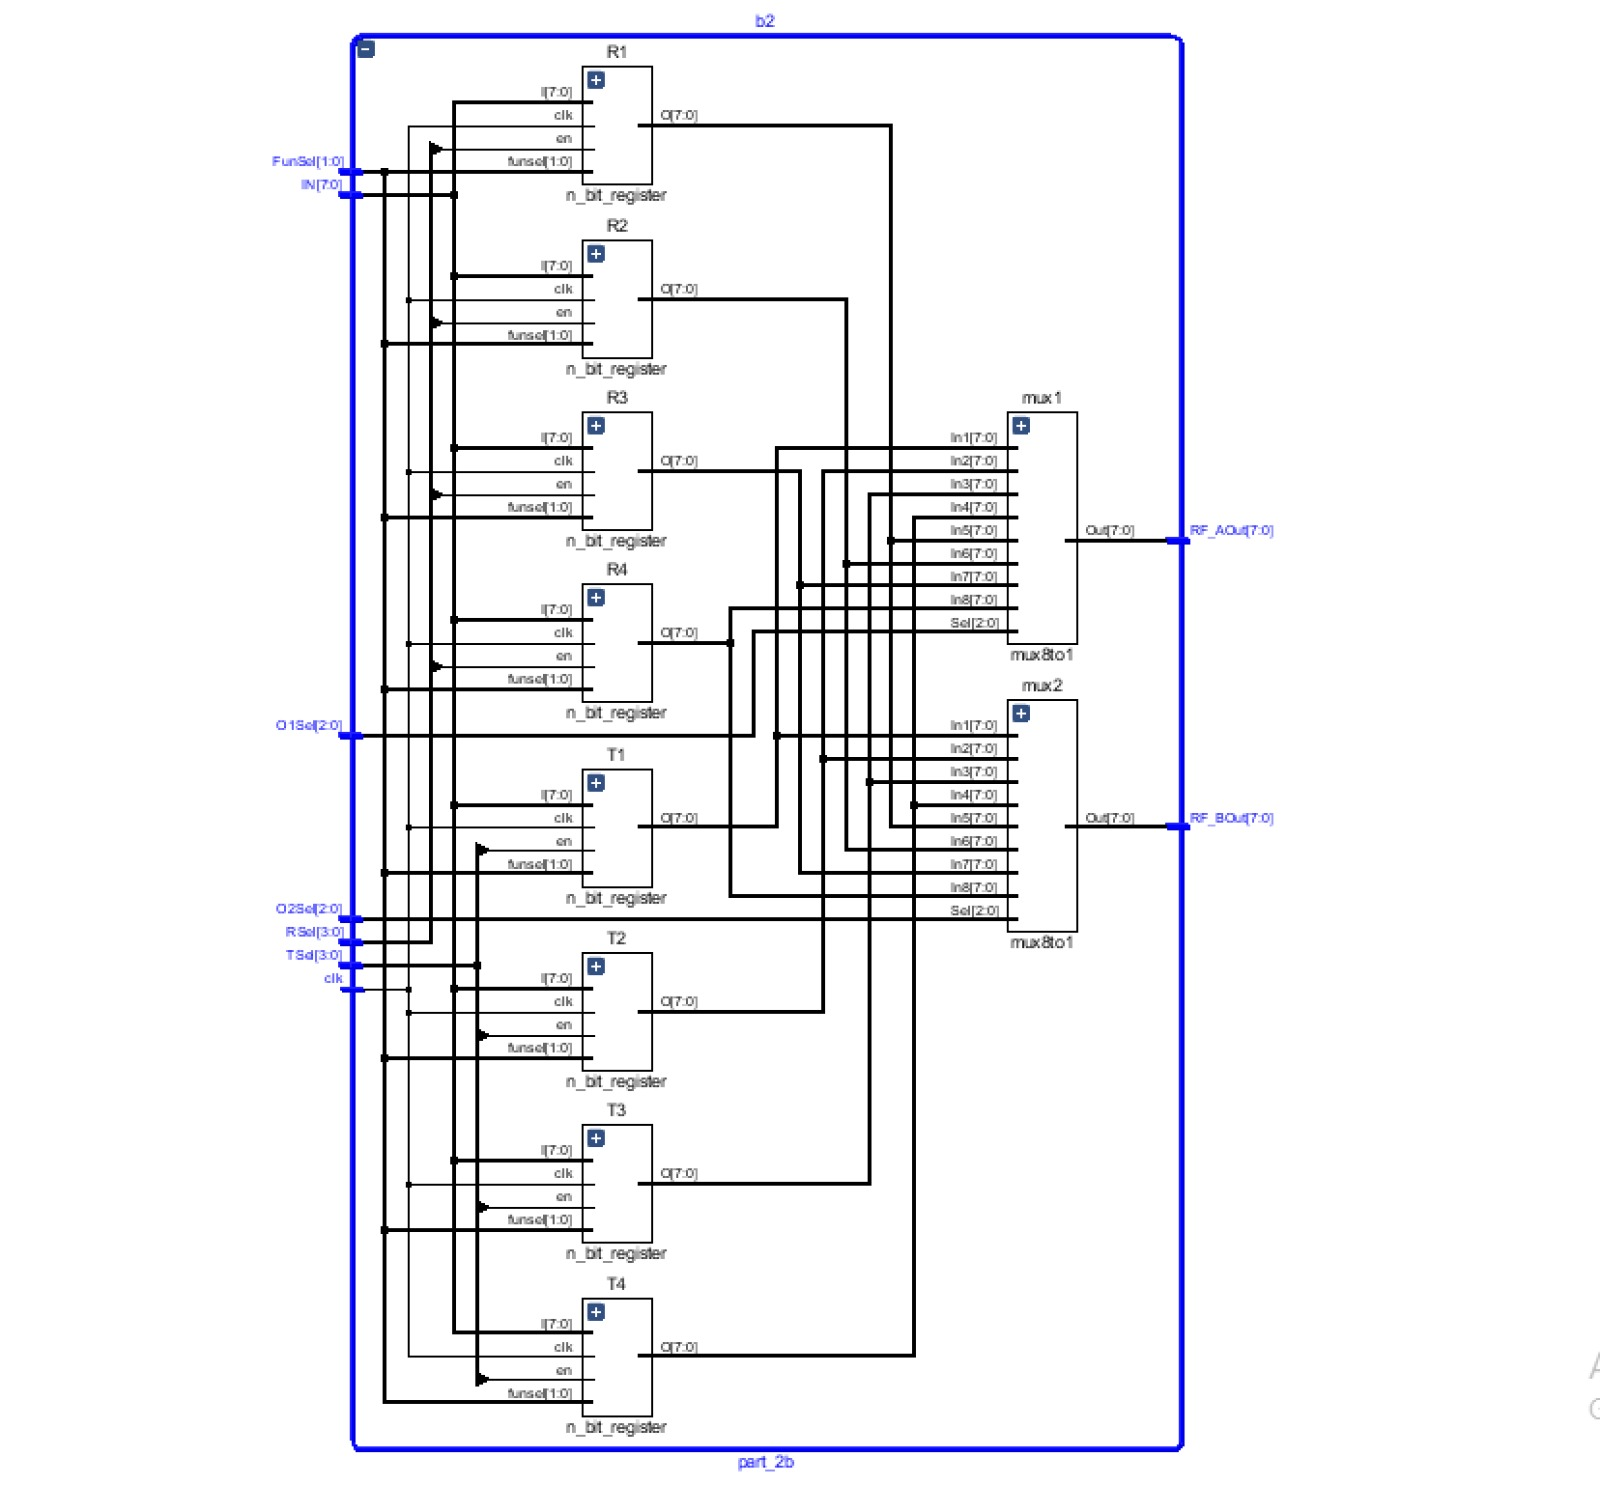
\includegraphics[width=4.5in]{2b.jpg}
    \caption{Figure for part-2b}
    \label{fig:part2b}
\end{figure}



\vspace{1cm}
Implementation of this module in Verilog shown in below:

\vspace{0.5cm}
\begin{lstlisting}
module part_2b(IN, O1Sel, O2Sel, FunSel, RSel, TSel, RF_AOut, RF_BOut,clk);
                  
        input [7:0] IN;
        input [2:0] O1Sel, O2Sel;
        input [1:0] FunSel;
        input [3:0] RSel, TSel;
        output reg[7:0] RF_AOut, RF_BOut;
        wire[7:0] mux1out, mux2out, R1O, R2O, R3O, R4O, T1O, T2O, T3O, T4O;
        input clk;
                    
        n_bit_register #(8) R1( RSel[3], FunSel, IN, R1O, clk);
        n_bit_register #(8) R2( RSel[2], FunSel, IN, R2O, clk);
        n_bit_register #(8) R3( RSel[1], FunSel, IN, R3O, clk);
        n_bit_register #(8) R4( RSel[0], FunSel, IN, R4O, clk);
        n_bit_register #(8) T1( TSel[3], FunSel, IN, T1O, clk);
        n_bit_register #(8) T2( TSel[2], FunSel, IN, T2O, clk);
        n_bit_register #(8) T3( TSel[1], FunSel, IN, T3O, clk);
        n_bit_register #(8) T4( TSel[0], FunSel, IN, T4O, clk);
                
       mux8to1 mux1(mux1out, O1Sel, T1O, T2O, T3O, T4O, R1O, R2O, R3O, R4O);
       mux8to1 mux2(mux2out, O2Sel, T1O, T2O, T3O, T4O, R1O, R2O, R3O, R4O);
        
        always @(*)
        
        begin
        RF_AOut=mux1out;
        RF_BOut=mux2out;
        end
                
        endmodule
\end{lstlisting}

\clearpage

We used two different modules in this module, these are the n bit register that we implement in the 1st part and and 8 to 1 mux.

\begin{figure}[H]
    \centering
    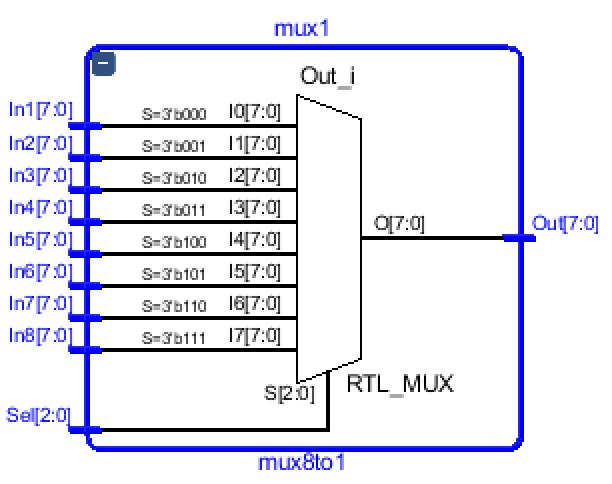
\includegraphics[width=3.5in]{8to1mux.jpg}
    \caption{8to1 mux}
    \label{fig:8to1mux}
\end{figure}

Code for mux 8to1 module:

\begin{lstlisting}
module mux8to1( Out, Sel, In1, In2, In3, In4, In5, In6, In7, In8); 
input [7:0]  In1, In2, In3, In4, In5, In6, In7, In8; 
input [2:0] Sel;
output [7:0] Out; 

reg [7:0] Out; 
always @ (*) 
begin 
 case (Sel) 
  3'b000 : Out = In1; 
  3'b001 : Out = In2; 
  3'b010 : Out = In3; 
  3'b011 : Out = In4; 
  3'b100 : Out = In5; 
  3'b101 : Out = In6; 
  3'b110 : Out = In7; 
  3'b111 : Out = In8; 

  default : Out = 8'bx; 
 endcase 
end  
endmodule\end{lstlisting}



\clearpage

\subsubsection{Part-2c)}
This ARF module has several inputs: 
\begin{itemize}
    \item It takes in a clock signal clk.
    \item an 8-bit input data signal inData.
    \item 2-bit function select signal FunSel.
    \item 4-bit register select signal RSel, selects the address register to access (i.e., PC, AR, SP, or PCPast). 
    \item 2-bit output A select signal OutASel.
    \item  2-bit output B select signal OutBSel.
\end{itemize}

Module has four 8-bit n-bit registers for each address register, namely PC, AR, SP, and PCPast. The module has two 4-to-1 multiplexers (amux and bmux) for selecting the output signals ARF\_AOut and ARF\_BOut, respectively. The OutASel and OutBSel signals are used to select the source of the output signals, which can be one of the four registers (AR, SP, PCPast, and PC).
The FunSel signal is used to control the operation of the n-bit registers. The possible operations are 00 (reset), 01 (load), 10 (decrement), and 11 (increment). The output signals of the n-bit registers are connected to the multiplexers, which select the appropriate output signal based on the OutASel and OutBSel signals.

\begin{figure}[H]
    \centering
    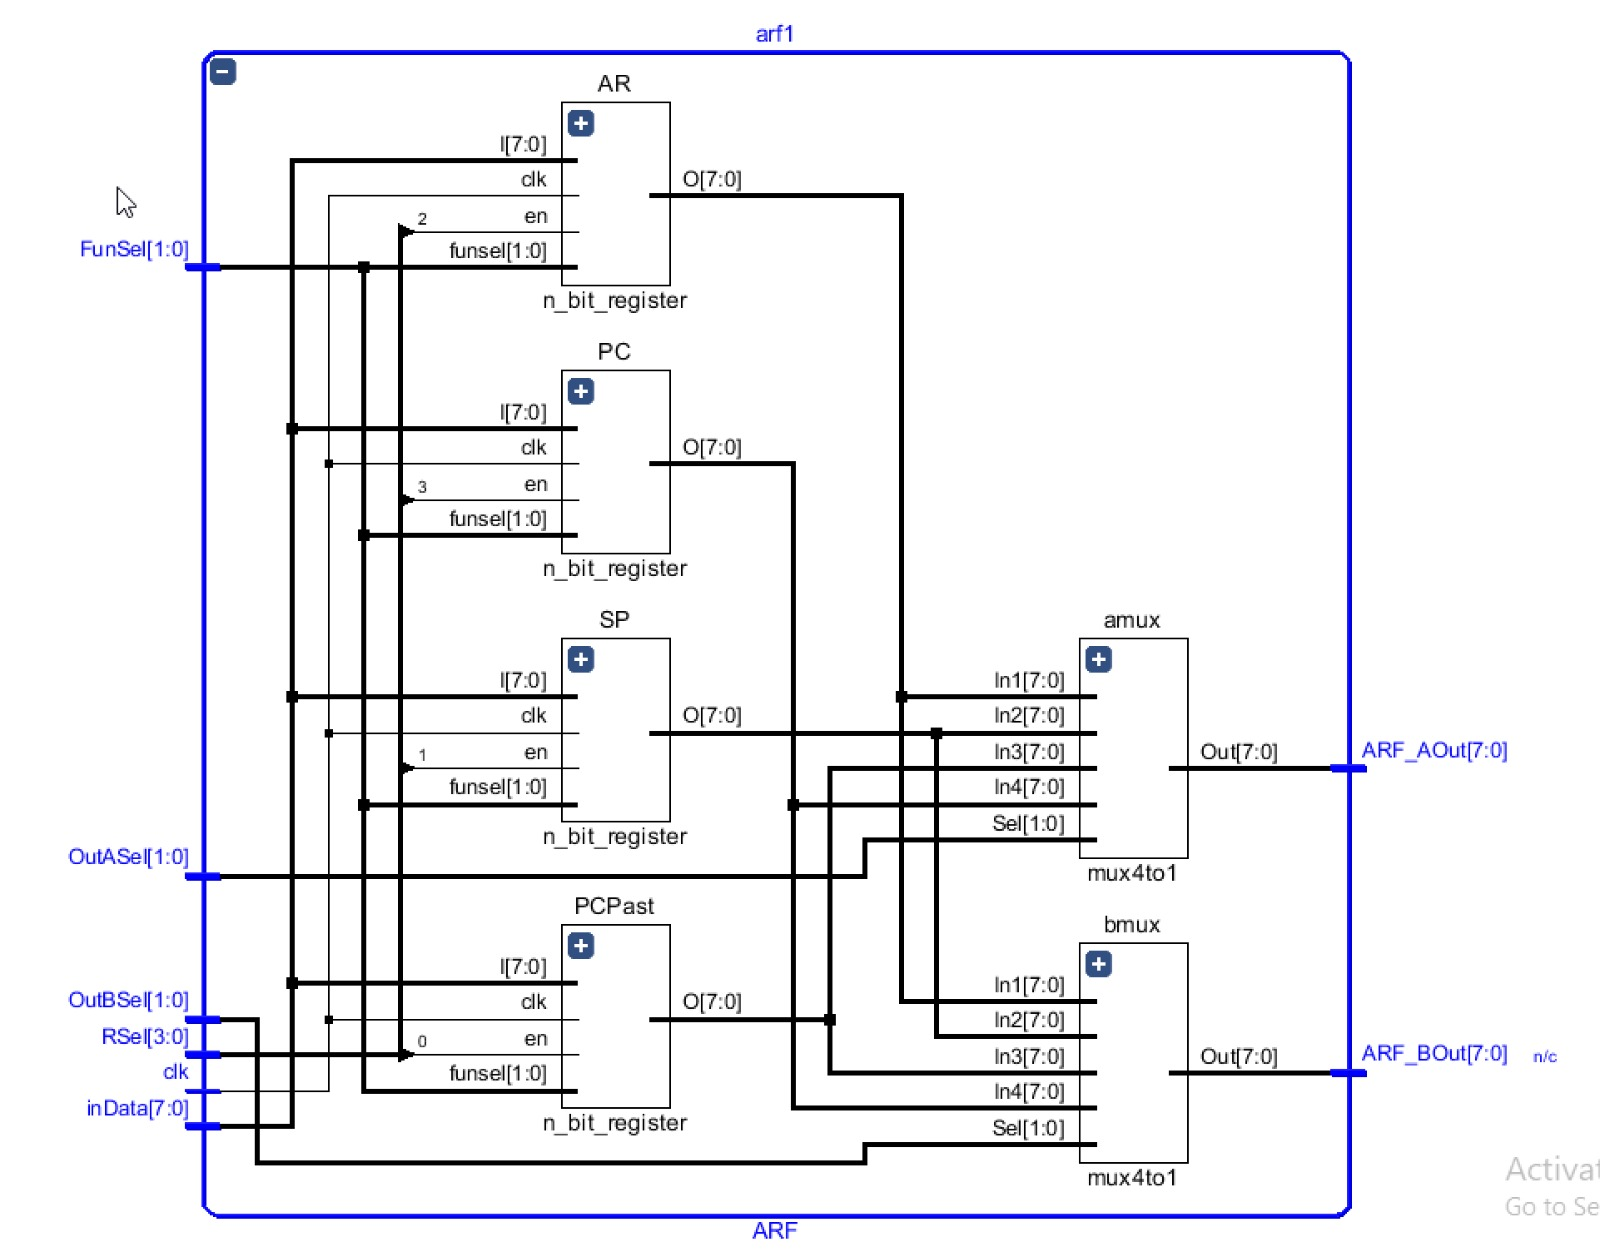
\includegraphics[width=5in]{2c.jpg}
    \caption{Figure for part-2c}
    \label{fig:part2c}
\end{figure}

\clearpage

Implementation of this module in Verilog shown in below:

\vspace{0.4cm}
\begin{lstlisting}
module ARF( input clk,
            input [7:0] inData, 
            input [1:0] FunSel, 
            input [3:0] RSel, 
            input [1:0] OutASel, OutBSel,
            output [7:0] ARF_AOut, ARF_BOut
        );
          
            wire [7:0] PCOut, AROut, SPOut,PCPastOut; 
           //multiplexer output signals
        
    n_bit_register #(8) PC(RSel[3], FunSel, inData, PCOut, clk ); 
    n_bit_register #(8) AR(RSel[2], FunSel, inData, AROut, clk );
    n_bit_register #(8) SP(RSel[1], FunSel, inData, SPOut, clk ); 
    n_bit_register #(8) PCPast(RSel[0], FunSel, inData, PCPastOut, clk);
    //registers for each address register
    
  mux4to1 amux(ARF_AOut, OutASel, AROut, SPOut,  PCPastOut, PCOut);
   //mux for selecting OutA
  mux4to1 bmux(ARF_BOut, OutBSel, AROut, SPOut,  PCPastOut, PCOut);
   //mux for selecting OutB

   
        endmodule
    
\end{lstlisting}

\clearpage

\subsection{Part-3}
This code represents an Arithmetic Logic Unit (ALU) in Verilog. The ALU performs various arithmetic and logical operations on two input values A and B based on the function code FunSel, and produces an output value OutAlu and several flags. Inputs of this ALU are:
\begin{itemize}
\item A: an 8-bit signed input
\item B: an 8-bit signed input
\item FunSel: a 4-bit input used to select the operation to be performed on A and B. The possible values of FunSel and their corresponding operations are:
   \begin{itemize}   
    \item 4'b0000: set OutAlu to A (no operation)
    \item 4'b0001: set OutAlu to B (no operation)
    \item4'b0010: set OutAlu to the bitwise NOT of A
    \item 4'b0011: set OutAlu to the bitwise NOT of B
    \item 4'b0100: set OutAlu to the sum of A and B
    \item 4'b0101: set OutAlu to the difference between A and B
    \item 4'b0110: compare A and B and set OutAlu to 0 or A depending on the result
    \item 4'b0111: set OutAlu to the logical AND of A and B
    \item 4’b1000: set OutAlu to the logical OR of A and B
    \item 4’b1001: set OutAlu to the logical NAND of A and B
    \item 4’b1010: set OutAlu to the logical XOR of A and B
    \item 4’b1011: set OutAlu to the Logical Shift Left of A
    \item 4’b1100: set OutAlu to the Logical Shift Right of A
    \item 4’b1101: set OutAlu to the Arithmetic Shift Left of A
    \item 4’b1110: set OutAlu to the Arithmetic Shift Right of A
    \item 4’b1111: set OutAlu to the Circular Shift Right of A
   \end{itemize}
\item CarryFlag: a single bit input used for the carry flag for the further operation
The outputs of the ALU are OutAlu (an 8-bit signed value representing the result of the operation), and Flag (a 4-bit vector containing various flags indicating the result of the operation). The flags are:
   \begin{itemize}
   \item Flag[0]: Overflow flag (set if signed addition or subtraction overflows)
   \item Flag[1]: Negative flag (set if result is negative)
   \item Flag[2]: Carry flag (set if there is a carry-out or borrow from the most significant bit)
   \item Flag[3]: Zero flag (set if result is zero)
   \end{itemize}
   The ALU is implemented using a case statement that selects the appropriate operation based on the value of FunSel. Inside each case, the appropriate operation is performed on A and B, and the result is assigned to OutAlu. Various flags are set based on the result of the operation.
\end{itemize}   

\begin{figure}[H]
    \centering
    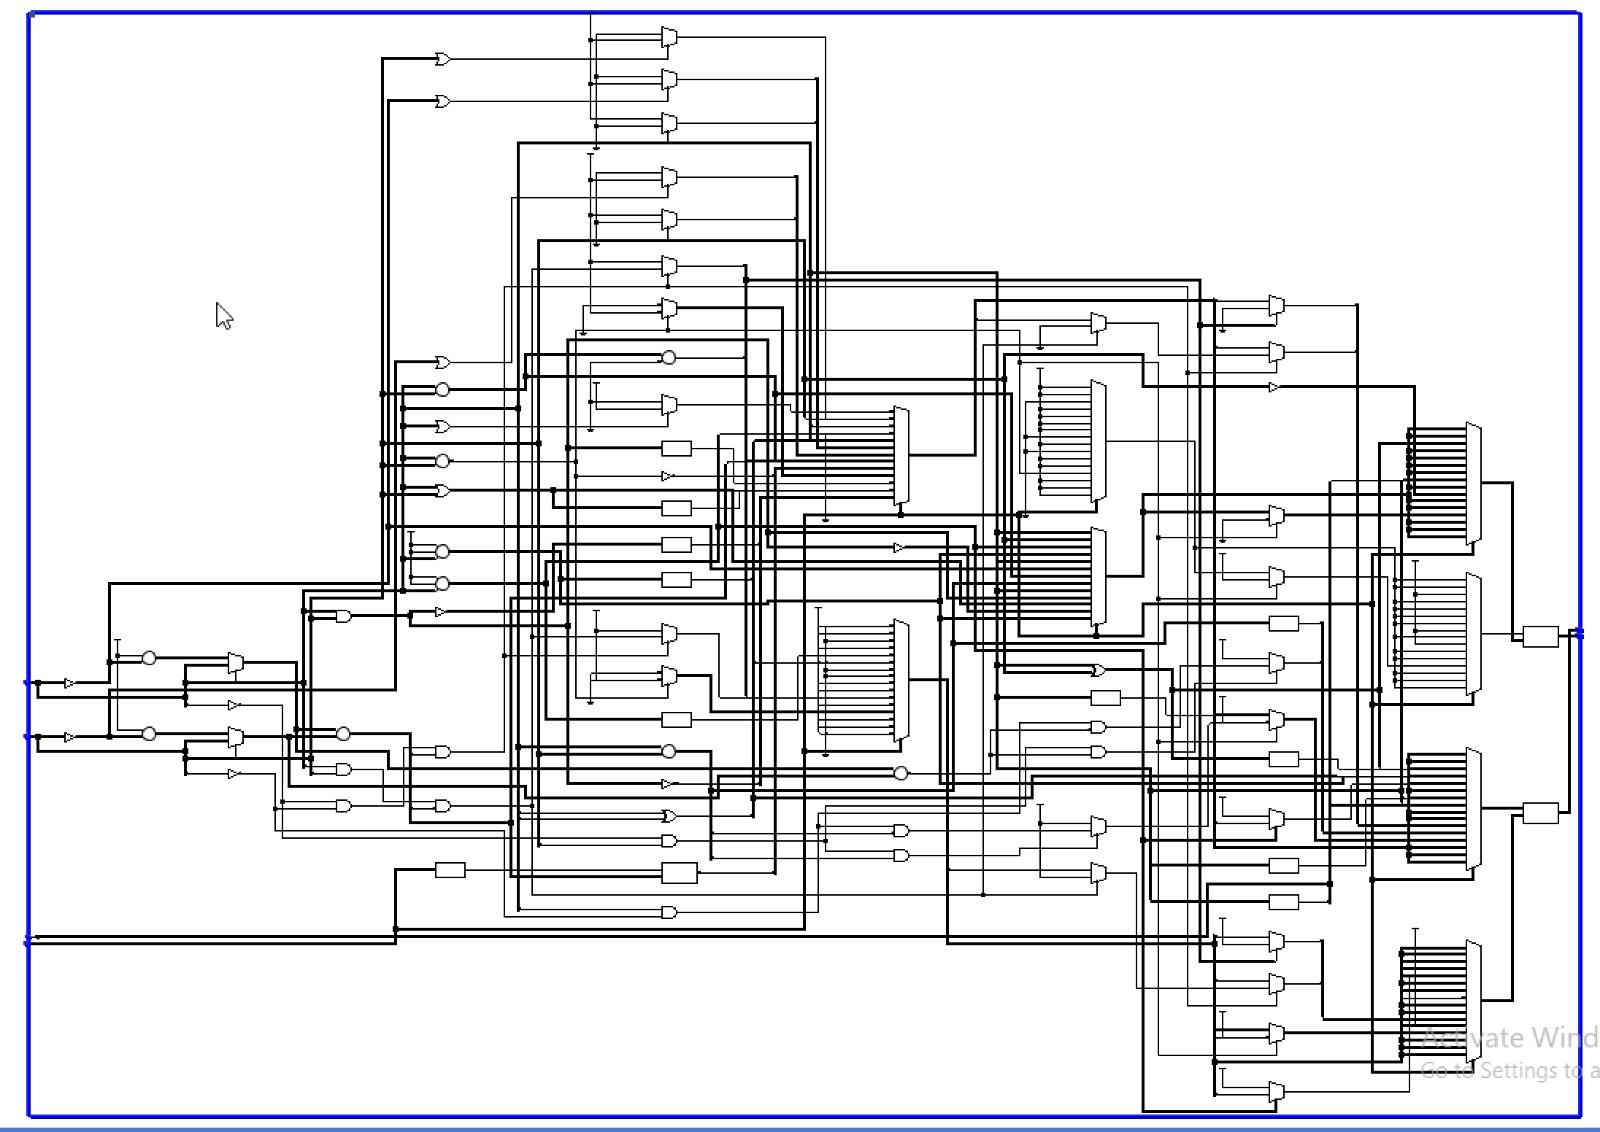
\includegraphics[width=5in]{3.jpg}
    \caption{Figure for part-3}
    \label{fig:part3}
\end{figure}

\vspace{1cm}
Implementation of this module in Verilog shown in below:
 
\vspace{0.5cm}
\begin{lstlisting}
module ALU( 

input [7:0]A, // signed
input [7:0]B, // signed
input[3:0] FunSel,
input CarryFlag,
output reg  [7:0] OutAlu, // signed
output reg [3:0]Flag
);
reg[7:0] sum, dif, negA, negB, log;
reg[8:0] temp;

always @(*)
begin
case(FunSel)
     4'b0000:  begin 
            OutAlu = A; 
            if(A) begin Flag[3]=0; end
            else begin Flag[3]=1; end
            if (A[7]) begin  Flag[1]=1;  end
            else begin Flag[1]=0; end
             end
     4'b0001: begin
           if(B) begin Flag[3]=0; end
           else begin Flag[3]=1; end
           if(B[7]) begin Flag[1]=1; end
           else begin Flag[1]=0; end
           OutAlu = B ;
           end
     4'b0010: begin
            OutAlu = ~A;
            if(~A) begin Flag[3]=0; end
            else begin Flag[3]=1; end
            if(~A[7]) Flag[1]=1;
            else Flag[1]=0;
            end
     4'b0011: begin
           OutAlu <= ~B;
            if(~B) begin Flag[3]=0; end
            else begin Flag[3]=1; end
            if(~B[7]) begin Flag[1]=1; end
            else begin Flag[1]=0; end
            end
     4'b0100:  begin
           OutAlu = A+B;
           sum = A+B;
           temp = A+B;  
           //check is Zero
           if((A+B)==8'd0) begin Flag[3]=1; end
           else begin Flag[3]<=0;end   
           Flag[2]= temp[7];      //carry flag
           if (A[7]) begin negA = ~A + 8'd1; end
           else negA = A;  //check negative(for signed)
           if(B[7]) begin  negB = ~B +8'd1; end
           else negB=B;
           sum = negA+negB;
           Flag[1]=sum[7];   
           if (~A[7] && ~B[7] && sum[7]) begin Flag[0]=1;
           end //pos+pos =neg      
           else if(A[7] && B[7] && ~sum[7]) begin Flag[0]=1; 
           end     //neg + neg = pos
           else begin Flag[0]<=0; end
           end         //check overflow 
     4'b0101:  begin
           OutAlu = A-B;
           dif = A-B;
           temp = A-B;    //check Zero Flag
           if(dif==8'd0) begin Flag[3]<=1; end
           else begin Flag[3]<=0; end
           Flag[2]= ~temp[8];      //Carry(borrow)
           if (A[7]) begin negA = ~A + 8'd1; end
           else negA = A;    //Negative Flag
           if(B[7]) begin  negB = ~B +8'd1; end
           else negB=B;
           dif = negA-negB;
           Flag[1]=sum[7];
           if (~A[7] && B[7] && dif[7]) begin Flag[0]<=1; 
           end//pos-neg =neg
           else if(A[7] && ~B[7] && ~dif[7]) begin Flag[0]<=1;
           end      //neg - pos = pos
           else begin Flag[0]<=0; end
           end
     4'b0110:  begin //COMPARE
           dif=A-B;
           temp=A-B;            
            if(temp[8]) begin
            OutAlu=A; 
            if(A==8'd0) begin Flag[3]<=1; end
            else begin Flag[3]<=0; end
            Flag[2]=0;
            Flag[1]=0;
            Flag[0]=0;
            end
            else begin
            OutAlu<=8'd0;    //negative flag
            Flag[1]<=1;      //carry flag
            Flag[2]=1;       //zero flag
            Flag[3]<=1;      //overflow
            if (~A[7] && B[7] && dif[7]) begin Flag[0]<=1; 
            end      //pos-neg =neg
            else if(A[7] && ~B[7] && ~dif[7]) begin Flag[0]<=1;
            end      //neg - pos = pos
            else begin Flag[0]<=0; end
            end
     end      
     4'b0111: begin     //Logical and
           OutAlu = A & B;
           log = A&B;
           if(log==8'd0) begin Flag[3]=1; end
           else begin Flag[3]=0; end
           if(log[7])begin  Flag[1]=1; end
           else begin Flag[1]=0; end
           end
     4'b1000: begin     //Logical or
           OutAlu = A | B;
           log = A|B;
           if((A|B)==8'd0) begin Flag[3]=1; end
           else begin Flag[3]=0; end
           if(log[7]) begin Flag[1]=1; end
           else begin Flag[1]=0; end
           end
     4'b1001: begin     //Logical nand
           OutAlu = ~(A & B);
           log = ~(A & B);
           if( log == 8'd0 ) begin Flag[3]=1; end
           else begin Flag[3]=0; end
           if(log[7]) begin Flag[1]=1; end
           else begin Flag[1]=0; end
           end
     4'b1010:begin    //Logical xor
           OutAlu <= A ^ B;
           log = A ^ B;
           if(log==8'd0) begin Flag[3]<=1; end
           else begin  Flag[3]<=0; end
           if(log[7]) begin Flag[1]<=1; end
           else  begin Flag[1]<=0; end
           end  //carry
     4'b1011: begin    //Logical shift left
           Flag[2]=A[7]; //set the carry flag
           log = (A<<1);
           OutAlu = log;
           if((A<<1)==8'd0)begin Flag[3]<=1; end
           else begin Flag[3]<=0; end
           if(log[7]) begin Flag[1]<=1; end
           else begin Flag[1]<=0; end
          end
     4'b1100: begin    //Logical shift right 
           Flag[2]<=A[0];
           log= (A>>1);
           OutAlu =log;
           if((A>>1)==8'd0) begin Flag[3]<=1; end
           else  begin Flag[3]=0; end
           if(log[7]) begin Flag[1]=1; end
           else begin Flag[1]=0; end
          end
     4'b1101: begin   //Arithmetic shift left
           log = (A<<1);
           OutAlu = log;
           if(log==8'd0)begin Flag[3]=1; end //overflow
           else begin Flag[3]=0; end
           if(A[6])begin Flag[1]=1; end
           else begin Flag[1]=0; end
           if (A[6]^A[7]) begin Flag[0] = 1; end
          end
     4'b1110: begin    //Arithmetic shift right
          OutAlu = {A[7],A[7:1]};
          if({A[7],A[7:1]}==8'd0)begin  Flag[3]<=1; end
          else begin Flag[3]<=0; end
          if(A[7]) begin Flag[1]<=1; end
          else begin Flag[1]<=0; end
        end
     4'b1111: begin    //Circular shift 
          OutAlu <={CarryFlag, A[7:1]};
          Flag[2] <= A[0];  //flag kontrol
          if({CarryFlag, A[7:1]}==8'd0)begin  Flag[3]<=1; end
          else begin Flag[3]<=0; end
          if(CarryFlag)begin  Flag[1]<=1; end
          else begin Flag[1]<=0; end
        end       
endcase
end

endmodule
\end{lstlisting}

\clearpage

\subsection{Part-4}
In part 4 we use 7 different modules and we connect the outputs and input to each other. 
The modules are:
\begin{itemize}
    \item Module two\_a (part 2a)
    \item Mux 4 to 1
    \item Module part\_2b (part 2b)
    \item Mux 2 to 1 
    \item Module ALU (part 3)
    \item Memory (given module)
    \item Module ARF (part 2c)
\end{itemize}

\begin{figure}[H]
    \centering
    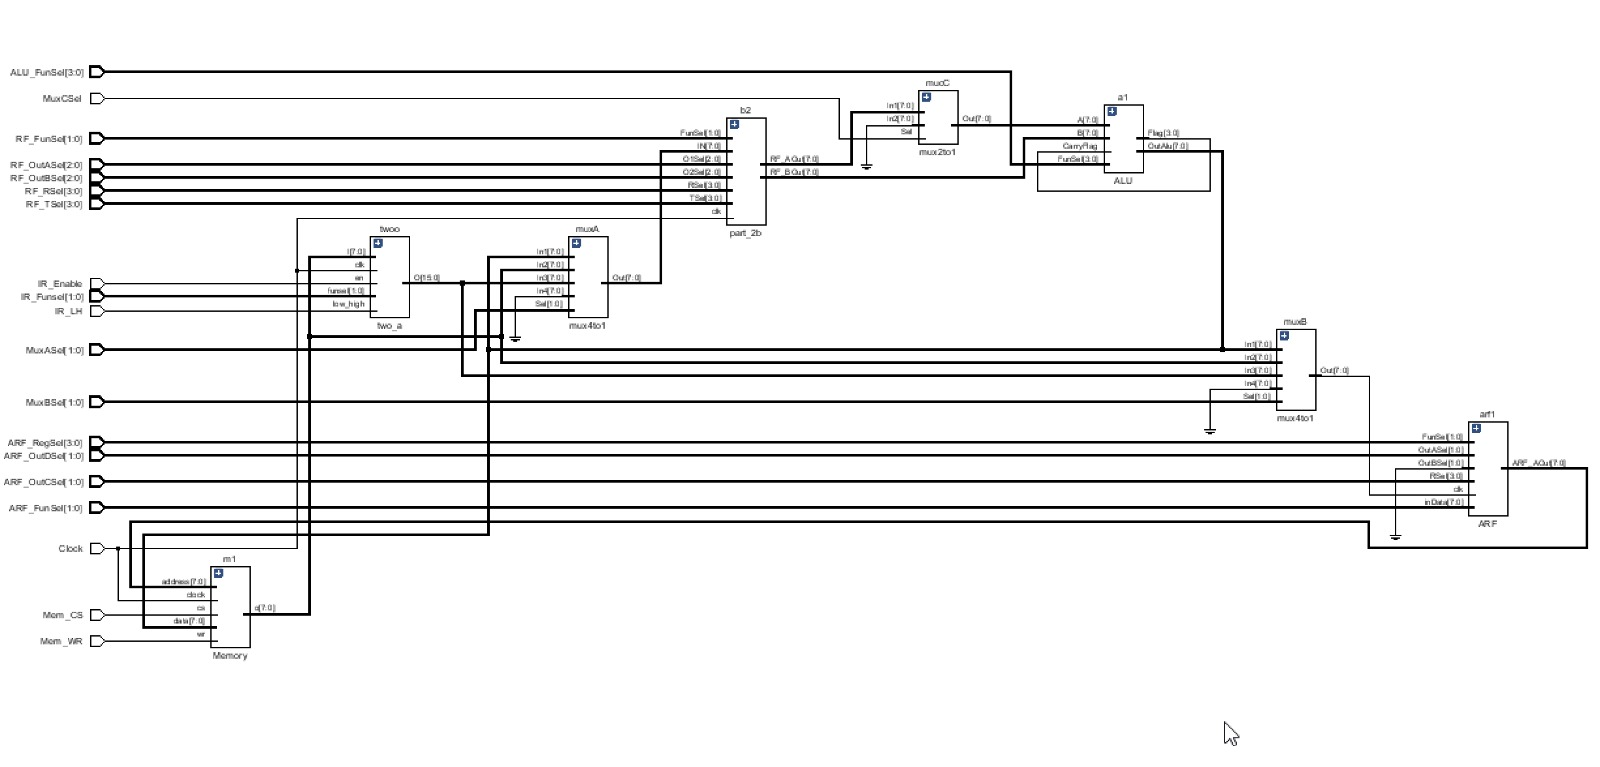
\includegraphics[width=6in]{4.jpg}
    \caption{Caption}
    \label{fig:part4}
\end{figure}
    
\clearpage

\begin{lstlisting}
module ALU_System(
    input [2:0]RF_OutASel,
    input [2:0]RF_OutBSel,
    input [1:0]RF_FunSel,
    input [3:0]RF_RSel,
    input [3:0]RF_TSel,
    input [3:0]ALU_FunSel,
    input [1:0]ARF_OutCSel,
    input [1:0]ARF_OutDSel,
    input [1:0]ARF_FunSel,
    input [3:0]ARF_RegSel,
    input IR_LH,
    input IR_Enable,
    input [1:0]IR_Funsel,
    input Mem_WR,
    input Mem_CS,
    input [1:0]MuxASel,
    input [1:0]MuxBSel,
    input MuxCSel,
    input Clock
    );
    wire [7:0] MemoryOut, MuxAOut, MuxCOut, alu_input_b, ALUOut;
    wire [7:0] MuxBOut, ARF_COut, Address,AOut,BOut;
    wire [15:0]output_2a;
    wire [7:0]IROut;
    wire [3:0]ALUOutFlag;
 
Memory m1( Address, ALUOut, Mem_WR, Mem_CS, Clock, MemoryOut );
two_a twoo(IR_Enable, Clock ,IR_Funsel , MemoryOut, IR_LH, output_2a);
assign IROut = output_2a[7:0];
mux4to1 muxA(MuxAOut, MuxASel, ALUOut, MemoryOut, IROut, ARF_COut);
mux4to1 muxB(MuxBOut, MuxBSel, ALUOut, MemoryOut, IROut, ARF_COut); 
ARF arf1(Clock, MuxBOut, ARF_FunSel, ARF_RegSel, ARF_OutCSel, ARF_OutDSel, ARF_COut, Address);
part_2b b2(MuxAOut, RF_OutASel, RF_OutBSel, RF_FunSel, RF_RSel, RF_TSel, AOut, BOut, Clock);
mux2to1 mucC(MuxCOut, MuxCSel, AOut, ARF_COut);
ALU a1(MuxCOut, BOut, ALU_FunSel, ALUOutFlag[2], ALUOut, ALUOutFlag);
   
endmodule
\end{lstlisting}

\begin{figure}[H]
    \centering
    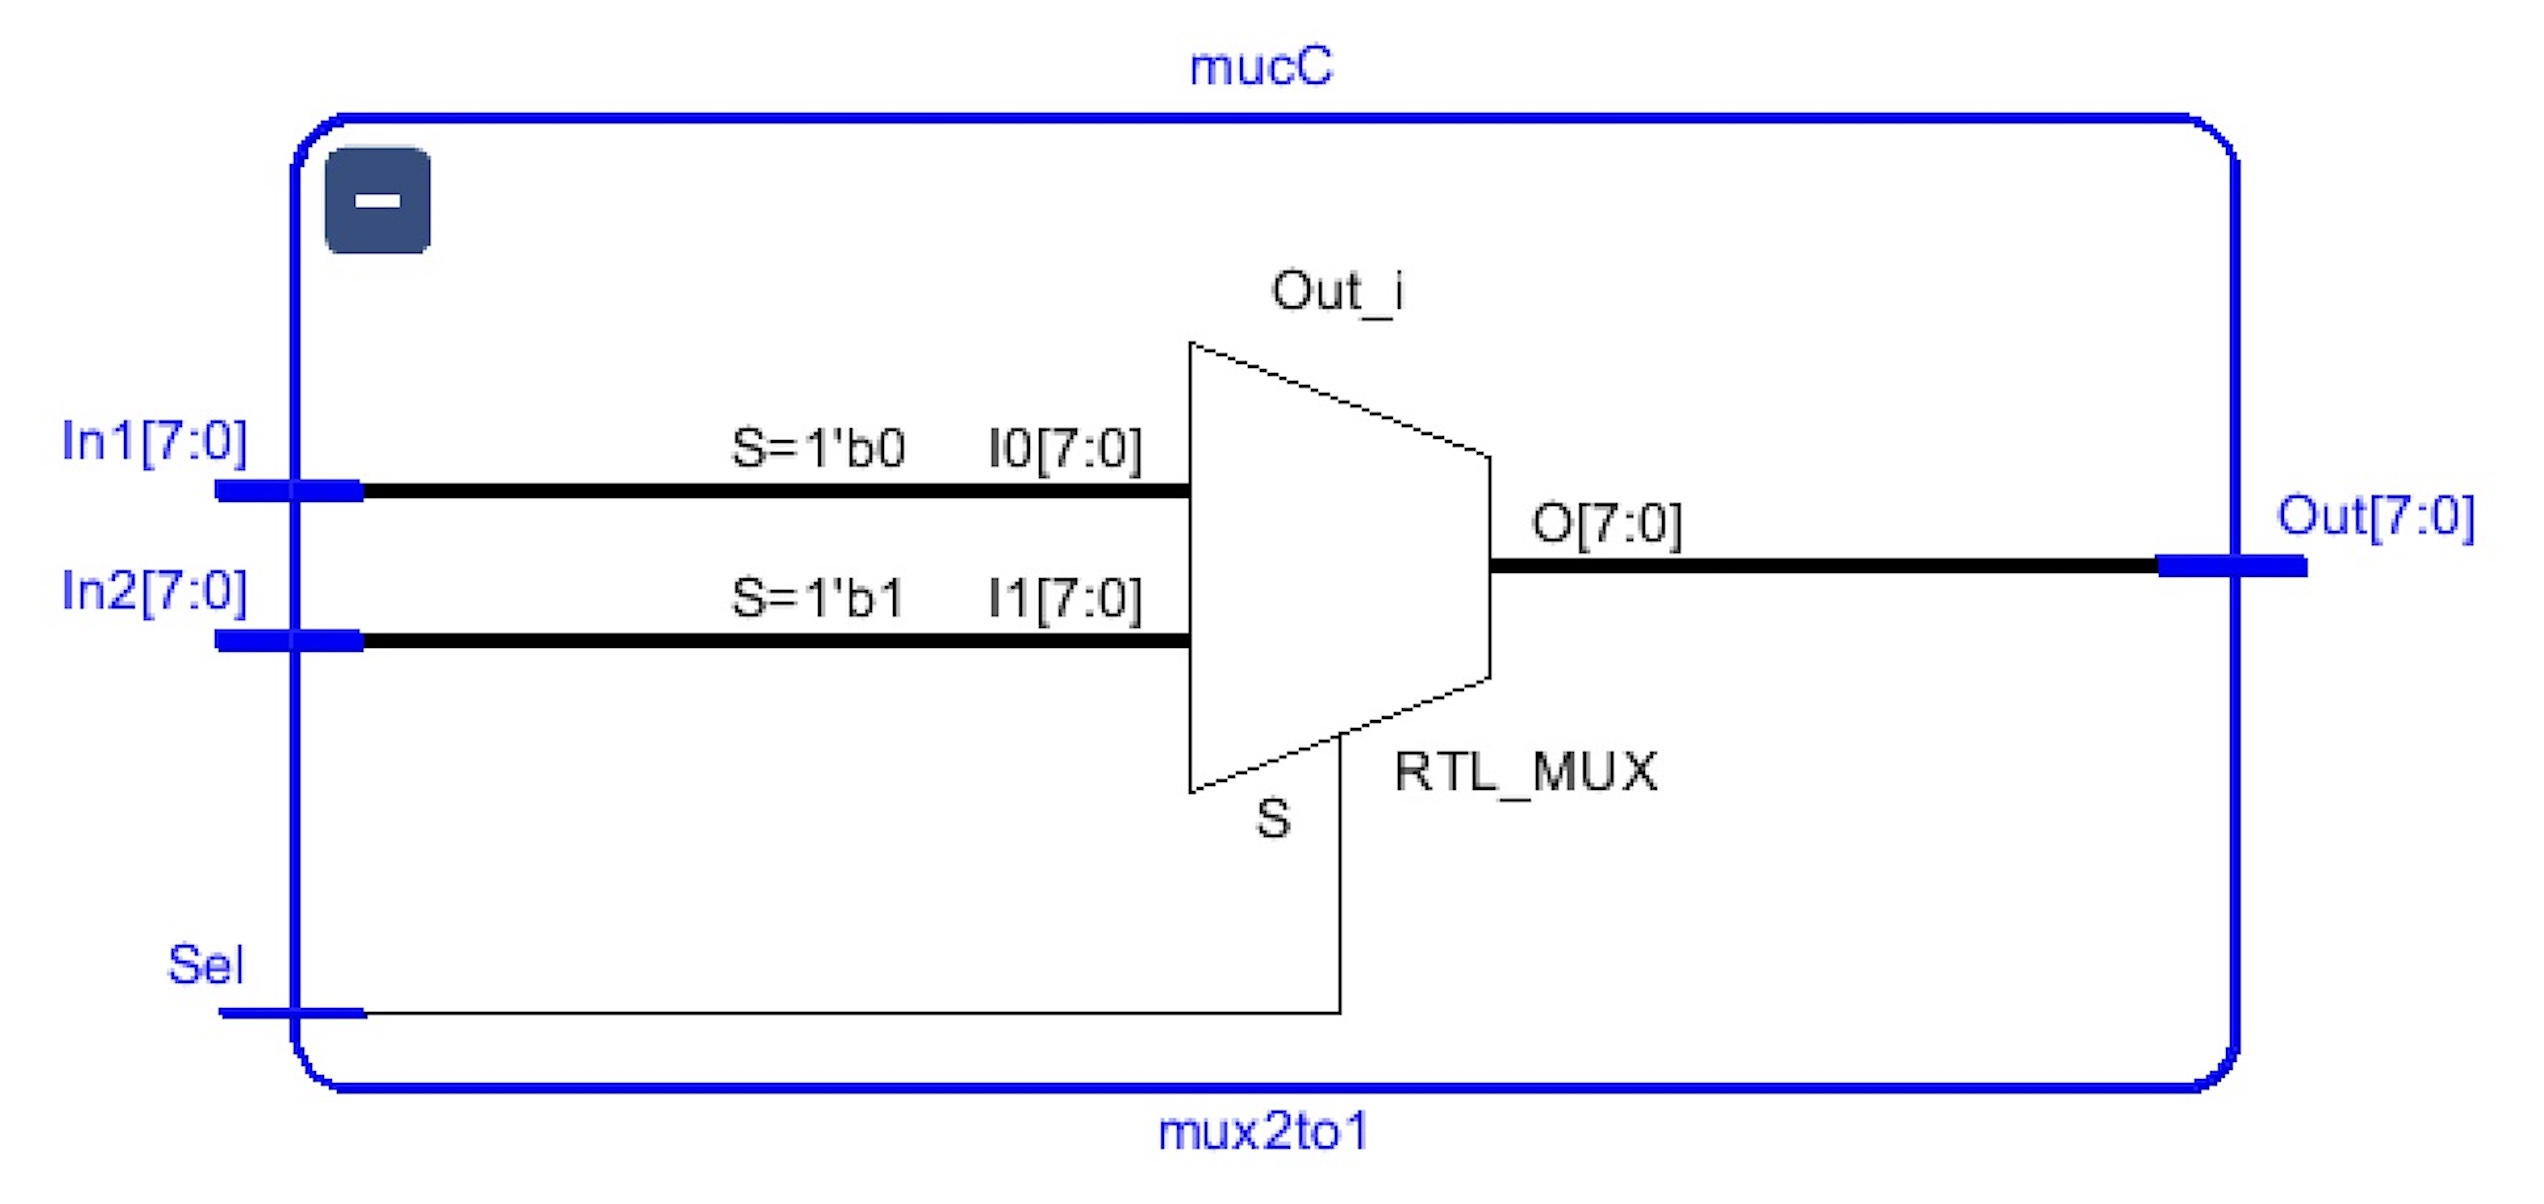
\includegraphics[width=6in]{part4mux.jpg}
    \caption{mux 2to1}
    \label{fig:mux1}
\end{figure}

\vspace{1.5cm}
\begin{figure}[H]
    \centering
    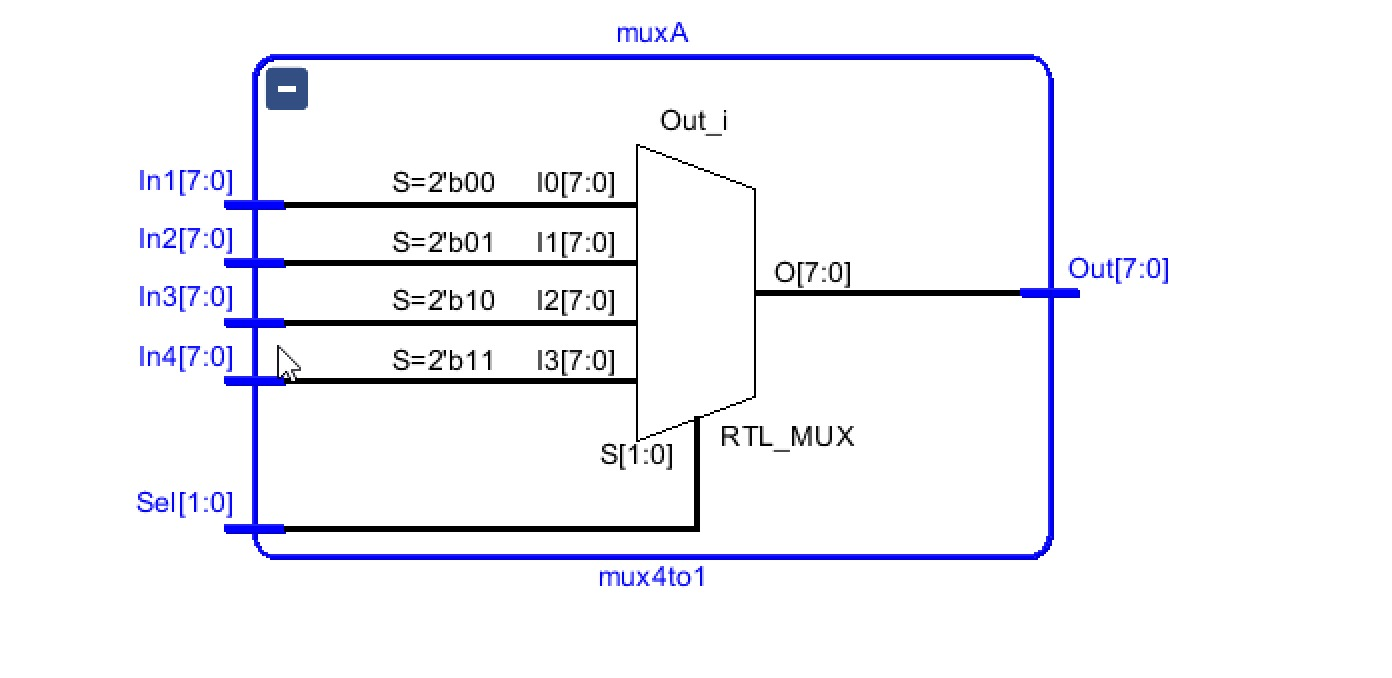
\includegraphics[width=6in]{part4mux2.jpg}
    \caption{mux 4to1}
    \label{fig:mux2}
\end{figure}



\clearpage

\section{Results}


 \subsection{Part-1}

In this testbench code for part 1 we use:

\begin{lstlisting}
    in = 8'b10111010;
    en=1; funsel = 2'd1; #50;
    //Values for test the load operation
    
    en=1; funsel = 2'd3; #50;
    en=1; funsel = 2'd2; #50;
    en=1; funsel = 2'd3; #50;
    //With this funsel values we test the increment and decrement operation.

    en=1; funsel = 2'd0; #50;
    //These values for testing the reset operations.

    en=0; funsel = 2'd3; #50;
    //For checking the enable inputs working correct.
    
    in = 8'b01010111;
    en=1; funsel = 2'd1; #50;
    //And control the load again.
\end{lstlisting}

Overall we did a test for every possible funsel and enable inputs.

\vspace{1cm}
\begin{figure}[H]
    \centering
    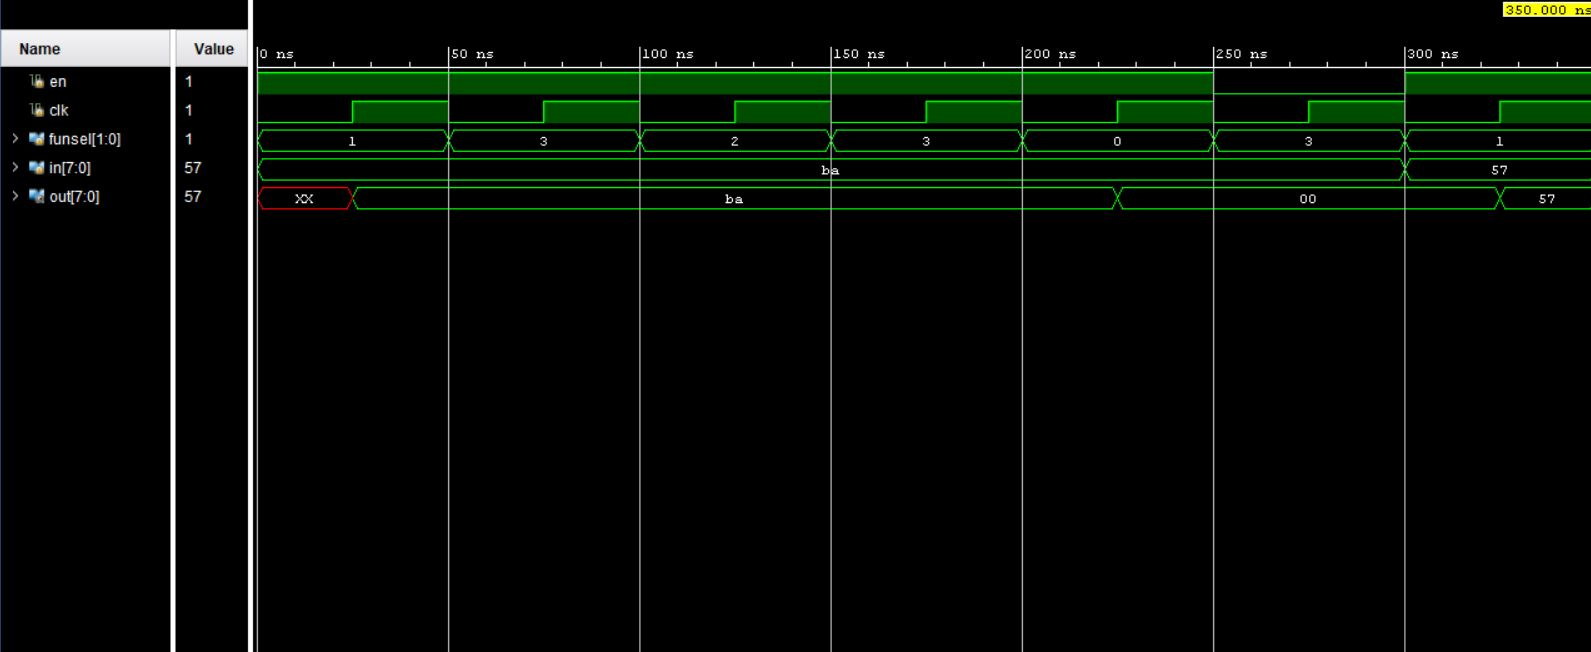
\includegraphics[width=6in]{r1.jpg}
    \caption{Simulation for part-1 }
    \label{fig:result1}
\end{figure}


\clearpage

 \subsection{Part-2}

\subsubsection{Part-2a)}

In the testbench code for part-2a we use these values:

\begin{lstlisting}
    clk=0;
    
    en = 1 ;  funsel[0] = 1  ; funsel[1] = 0  ; i = 8'b00001111 ;low_high = 0;#50;    
    // control to load to low part
    en = 1 ;  funsel[0] = 1  ; funsel[1] = 0  ; i = 8'b00011111 ;low_high = 1;#50;    
    // control to load to high part
    en = 1 ;  funsel[0] = 0  ; funsel[1] = 1  ; i = 8'b00001111 ;low_high = 0;#50;  
    // control to decrement operator
    en = 1 ;  funsel[0] = 1  ; funsel[1] = 1  ; i = 8'b00001111 ;low_high = 0;#50;    
    // control to increment operator
    en = 1 ;  funsel[0] = 0  ; funsel[1] = 0  ; i = 8'b00001111 ;low_high = 0;#50;    
    // control to reset
    en = 0 ;  funsel[0] = 1  ; funsel[1] = 1  ; i = 8'b00001111 ;low_high = 0;#50;    
    // to control that output is not changed when enable is 0
\end{lstlisting}

\begin{figure}[H]
    \centering
    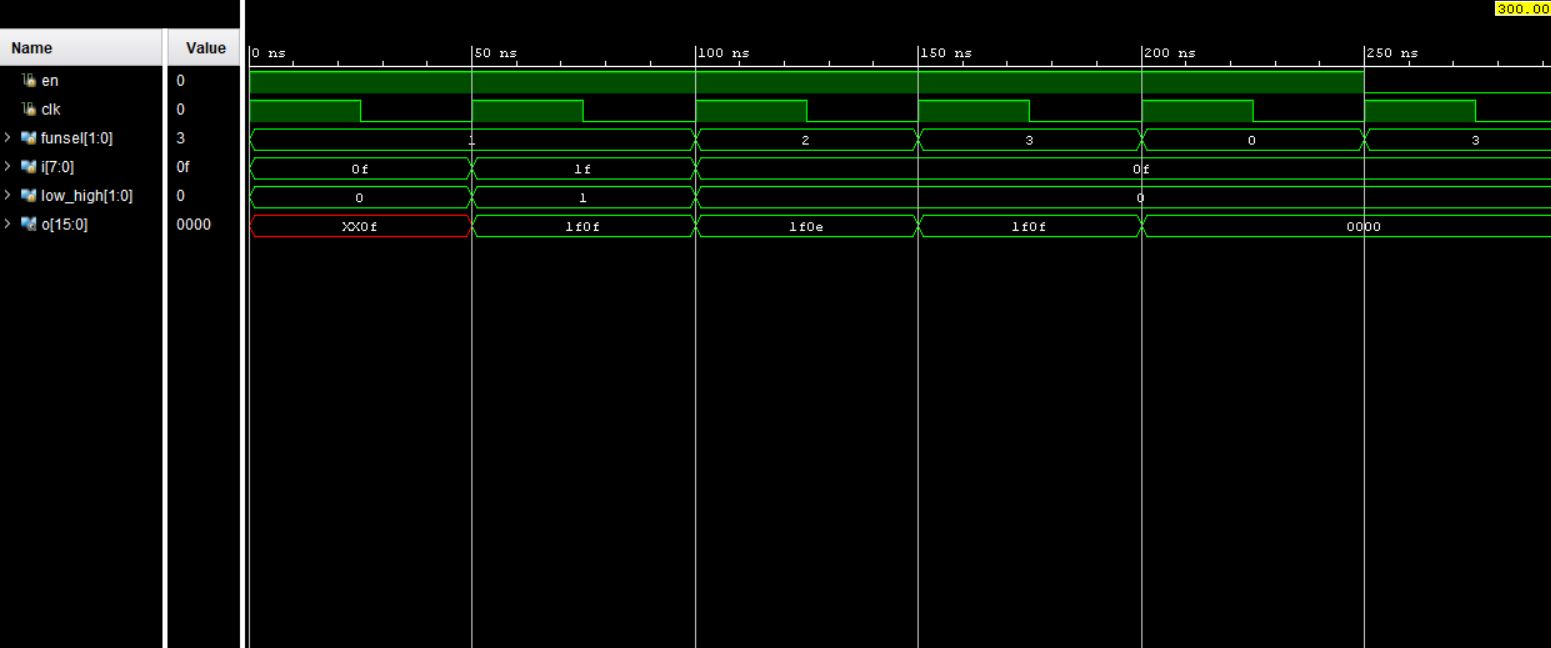
\includegraphics[width=6in]{r2a.jpg}
    \caption{Simulation for part-2a}
    \label{fig:result2a}
\end{figure}

\clearpage

\subsubsection{Part-2b)}

In the testbench code for part-2b we use these values:

\begin{lstlisting}
        IN = 8'b10101111;
        O1Sel = 3'd0; O2Sel = 3'd4; FunSel = 2'd1; RSel = 4'b1111; TSel = 4'b1111; #50;
        IN = 8'b10100011;
        O1Sel = 3'd0; O2Sel = 3'd4; FunSel = 2'd1; RSel = 4'b1111; TSel = 4'b1111; #50;
        IN = 8'b10100000;
        O1Sel = 3'd1; O2Sel = 3'd5; FunSel = 2'd1; RSel = 4'b1111; TSel = 4'b1111; #50;
        //to control load operation and possible delay.
        
        O1Sel = 3'd2; O2Sel = 3'd6; FunSel = 2'd3; RSel = 4'b1111; TSel = 4'b1111; #50;
        O1Sel = 3'd3; O2Sel = 3'd7; FunSel = 2'd3; RSel = 4'b1111; TSel = 4'b1111; #50;
        //to control increment operation .
        
        O1Sel = 3'd0; O2Sel = 3'd4; FunSel = 2'd2; RSel = 4'b1111; TSel = 4'b1111; #50;
        O1Sel = 3'd1; O2Sel = 3'd5; FunSel = 2'd2; RSel = 4'b1111; TSel = 4'b1111; #50;
        O1Sel = 3'd2; O2Sel = 3'd6; FunSel = 2'd2; RSel = 4'b0010; TSel = 4'b0010; #50;
        //to control decrement operation.
        
        O1Sel = 3'd3; O2Sel = 3'd7; FunSel = 2'd0; RSel = 4'b0001; TSel = 4'b0001; #50;
        //to control reset value.
        
        O1Sel = 3'd0; O2Sel = 3'd4; FunSel = 2'd3; RSel = 4'b0000; TSel = 4'b0000; #50;
        O1Sel = 3'd1; O2Sel = 3'd5; FunSel = 2'd3; RSel = 4'b0000; TSel = 4'b0000; #50;
        O1Sel = 3'd2; O2Sel = 3'd6; FunSel = 2'd3; RSel = 4'b0000; TSel = 4'b0000; #50;
        O1Sel = 3'd3; O2Sel = 3'd7; FunSel = 2'd1; RSel = 4'b0001; TSel = 4'b0001; #50;
        //to control, O1Sel, O2Sel RSel and TSel.
\end{lstlisting}

\begin{figure}[H]
    \centering
    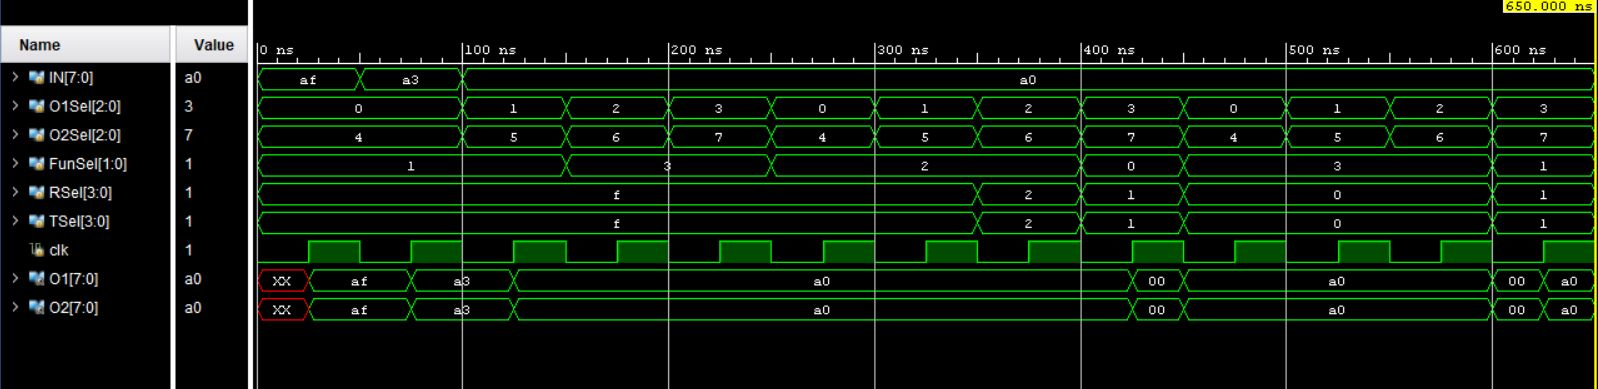
\includegraphics[width=6in]{r2bx.jpg}
    \caption{Simulation for part-2b}
    \label{fig:result2b}
\end{figure}


\subsubsection{Part-2c)}

In the testbench code for part-2c we use these values:

\begin{lstlisting}
i = 8'b10100101;
asel = 2'b00;   bsel = 2'b00;  funsel = 2'd1; Rsel = 4'b1111; #50;

i = 8'b10101111;
asel = 2'b00;   bsel = 2'b00 ;  funsel = 2'd1; Rsel = 4'b1111; #50;
//to control load operation.
asel = 2'b00;   bsel = 2'b00 ;  funsel = 2'd3; Rsel = 4'b1111; #50;
//to control increment operation.
asel = 2'b00;   bsel = 2'b00 ;  funsel = 2'd0; Rsel = 4'b1111; #50;
//to control reset input.

i = 8'b10100000;
asel = 2'b10;   bsel = 2'b00 ;  funsel = 2'd1; Rsel = 4'b1111; #50;
//to control load operation.
asel = 2'b00;   bsel = 2'b01 ;  funsel = 2'd2; Rsel = 4'b1111; #50;
//to control decrement operation.
asel = 2'b00;   bsel = 2'b00 ;  funsel = 2'd0; Rsel = 4'b0000; #50;
//to control Rsel input - enable.
asel = 2'b00;   bsel = 2'b01 ;  funsel = 2'd2; Rsel = 4'b1111; #50;
\end{lstlisting}

\begin{figure}[H]
    \centering
    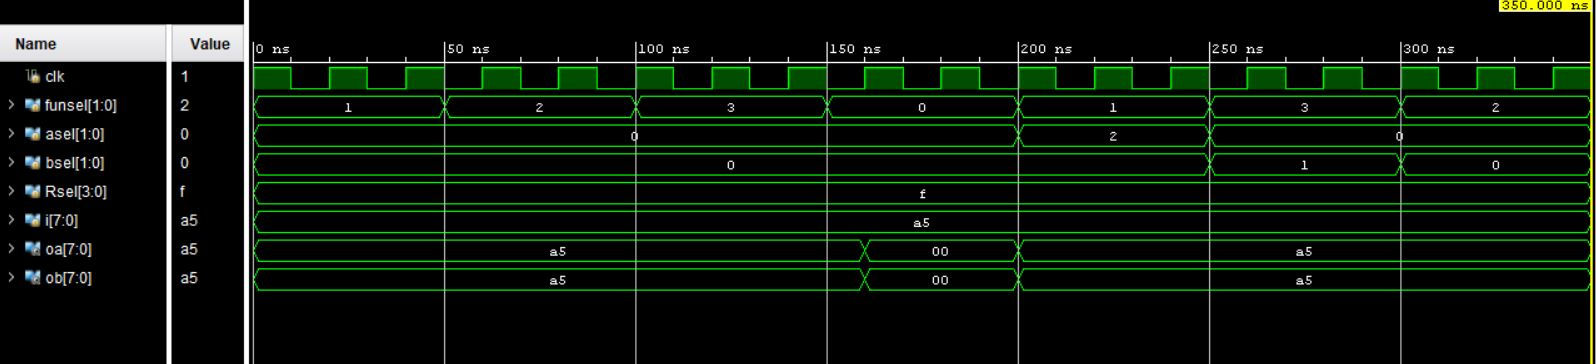
\includegraphics[width=6in]{r2c.jpg}
    \caption{Simulation for part-2c}
    \label{fig:result2c}
\end{figure}


\clearpage

 \subsection{Part-3}

In the testbench code for part-3 we use these test values:

\begin{lstlisting}
A=8'b00001010;
B=8'b00001001;
cflag= Flag[2]; Funsel=4'd0; #50;
cflag= Flag[2]; Funsel=4'd1; #50;
cflag= Flag[2]; Funsel=4'd2; #50;
cflag= Flag[2]; Funsel=4'd3; #50;
cflag= Flag[2]; Funsel=4'd4; #50;
cflag= Flag[2]; Funsel=4'd5; #50;
cflag= Flag[2]; Funsel=4'd7; #50;
cflag= Flag[2]; Funsel=4'd8; #50;
cflag= Flag[2]; Funsel=4'd9; #50;
cflag= Flag[2]; Funsel=4'd10; #50;
cflag= Flag[2]; Funsel=4'd11; #50;
cflag= Flag[2]; Funsel=4'd12; #50;
cflag= Flag[2]; Funsel=4'd13; #50;
cflag= Flag[2]; Funsel=4'd14; #50;
cflag= Flag[2]; Funsel=4'd15; #50;
cflag= Flag[2]; Funsel=4'd13; #50;
//to control every operations result we try the every possible funsel values. 

A=8'b10000000;
B=8'b10011111;
cflag= Flag[2];Funsel=4'd0; #50;
cflag= Flag[2];Funsel=4'd4; #50;
cflag= Flag[2];Funsel=4'd5; #50;
cflag= Flag[2];Funsel=4'd6; #50;
cflag= Flag[2];Funsel=4'd7; #50;
//signed values to control flags (overflow, negative).
\end{lstlisting}

\begin{figure}[H]
    \centering
    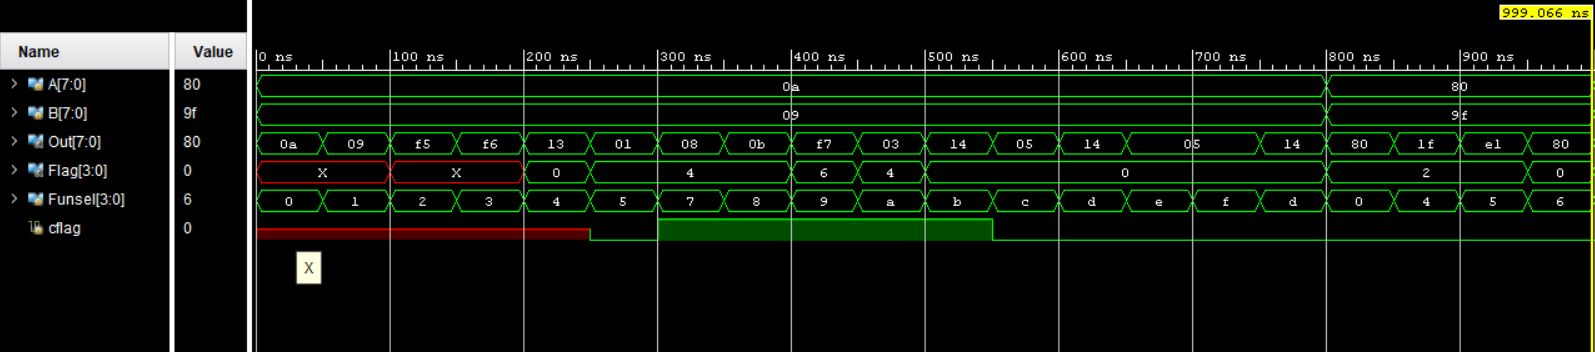
\includegraphics[width=6.2in]{r3.jpg}
    \caption{Simulation for part-3}
    \label{fig:result3}
\end{figure}

\clearpage

 \subsection{Part-4}
 
\begin{figure}[H]
    \centering
    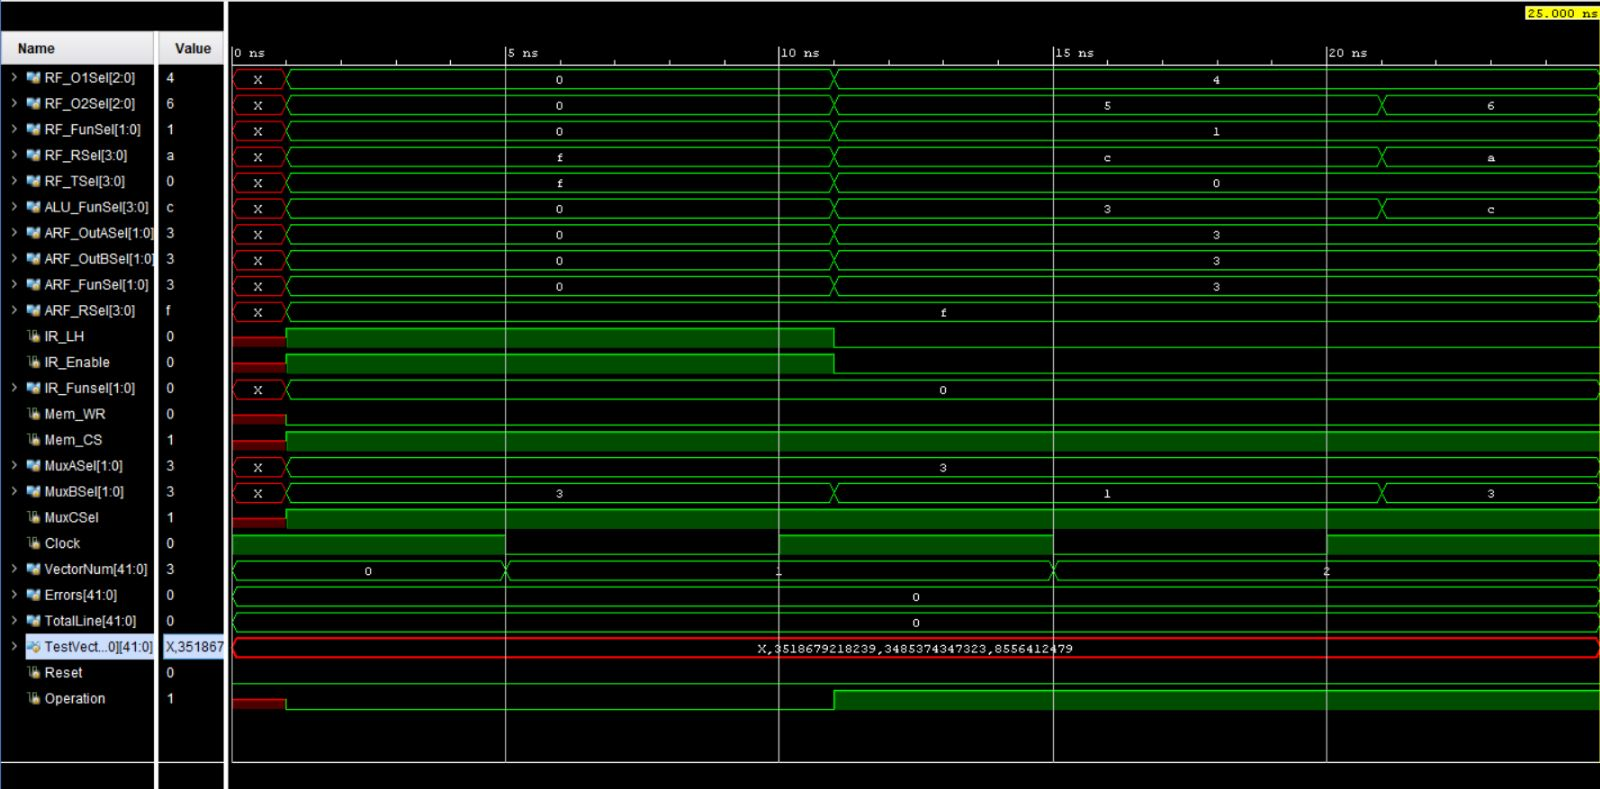
\includegraphics[width=6.2in]{r4.jpg}
    \caption{Simulation for part-4}
    \label{fig:result4}
\end{figure}

 \vspace{1cm}
\section{Task Distribution}
While doing the project, we mostly proceeded by sharing the parts. Çağla Mıdıklı worked mostly on Part-1, Part-2a, Part-3 and Part-4. Feyza Sarı worked mostly on Part-2b Part-3 and Part-4. Berna Karatay worked mostly on Part-2c and report writing part via latex.  




\end{document}